% !TeX root = ../Tempel-Daniel.tex
\chapter{LLM Benchmarks and Model Selection}
\label{chap:benchmarks}

Chapter~\ref{chap:local-llms} explained how model size, numerical representation and context requirements constrain local LLM deployment. These constraints determine which configurations are technically feasible, but not whether they can reliably perform the intended software-engineering tasks. Published benchmark results provide useful evidence, but only under particular tasks and evaluation conditions.

A benchmark is a standardised collection of tasks with a scoring procedure, whereas evaluation also includes the prompt, context, tools, execution limits and success criteria. Model selection uses this evidence to identify suitable candidates for a specific application. Frameworks such as HELM therefore evaluate language models across multiple scenarios and metrics rather than reducing capability to a single score \parencite{liang2022helm}.

In a practical deployment, candidate models should be compared within a fixed assistant architecture. Such results would describe their suitability for the target application rather than model capability in isolation. Candidates should also be treated as concrete deployment configurations, including the model version, quantization scheme, inference runtime, and runtime configuration intended for deployment.

\section{Evaluating software engineering capabilities}
\label{sec:engineering-capabilities}

Different benchmarks measure different capabilities, and their relevance depends on the target workload. General-purpose benchmarks such as MMLU-Pro evaluate knowledge and reasoning across multiple domains. MMLU-Pro was designed as a more difficult and less prompt-sensitive successor to MMLU, while Humanity's Last Exam was motivated partly by the increasing saturation of established academic benchmarks \parencite{wang2024mmlupro,phan2025hle}. Such evaluations provide evidence about broad reasoning ability but do not directly measure repository-level software engineering.

Coding benchmarks move closer to the intended workload. LiveCodeBench continuously incorporates recently published programming problems and evaluates capabilities including code generation, execution and self-repair \parencite{jain2024livecodebench}. Using recently published tasks can reduce contamination risk relative to static datasets, although their publication dates must still be considered in relation to the training cutoff of the evaluated model. Execution-based evaluation is particularly useful for programming because different implementations can be textually different while exhibiting the same correct behaviour.

Repository-level work introduces additional requirements such as code navigation, integration with existing components and regression control. SWE-Lancer contains more than 1,400 tasks originating from real freelance software-engineering work. Its independent engineering tasks are evaluated using end-to-end tests, while a separate category of managerial tasks requires choosing between technical implementation proposals \parencite{miserendino2025swelancer}.

Tool-based environment interaction represents another relevant evaluation dimension. Terminal-Bench 2.0 evaluates systems in command-line environments where they must inspect the environment, execute commands, observe results and complete multi-step tasks \parencite{merrill2026terminalbench}. This becomes relevant when an LLM is embedded into an interactive system rather than used only for single-response generation.

Figure~\ref{fig:evaluation-dimensions} relates these complementary benchmark dimensions to the representative assistant tasks that a deployment evaluation should cover.

\noindent\begin{minipage}{\linewidth}
\centering
% Trim only outer whitespace; preserve all labels and the explanatory footer.
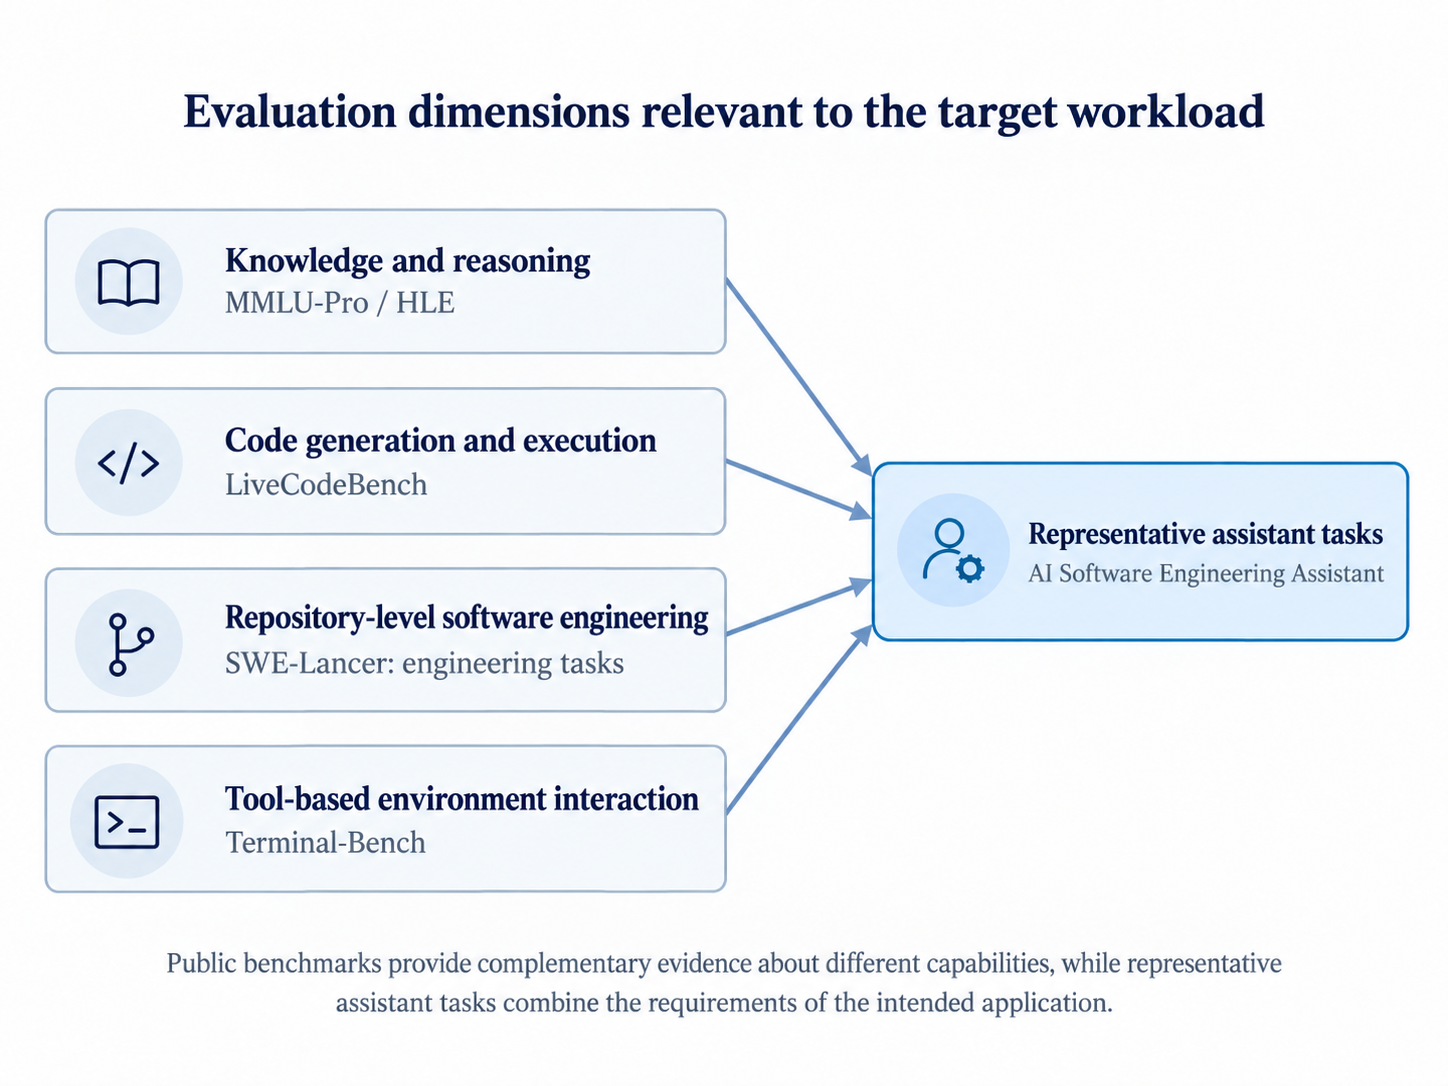
\includegraphics[width=14cm,trim=0 45bp 0 60bp,clip]{images/benchmark-evaluation-dimensions.png}
\captionsetup{hypcap=false}
\captionof{figure}{Evaluation dimensions relevant to the target workload of the AI Software Engineering Assistant. The dimensions overlap; the listed benchmarks are illustrative examples.}
\label{fig:evaluation-dimensions}
\end{minipage}

Figure~\ref{fig:evaluation-factors} shows why measured performance depends on the assistant configuration and execution conditions as well as the model. The evaluation harness initialises the task environment, executes the assistant under defined limits and records the resulting actions and outputs. The evaluator and acceptance tests then determine whether the resulting solution satisfies the task requirements.

\noindent\begin{minipage}{\linewidth}
\centering
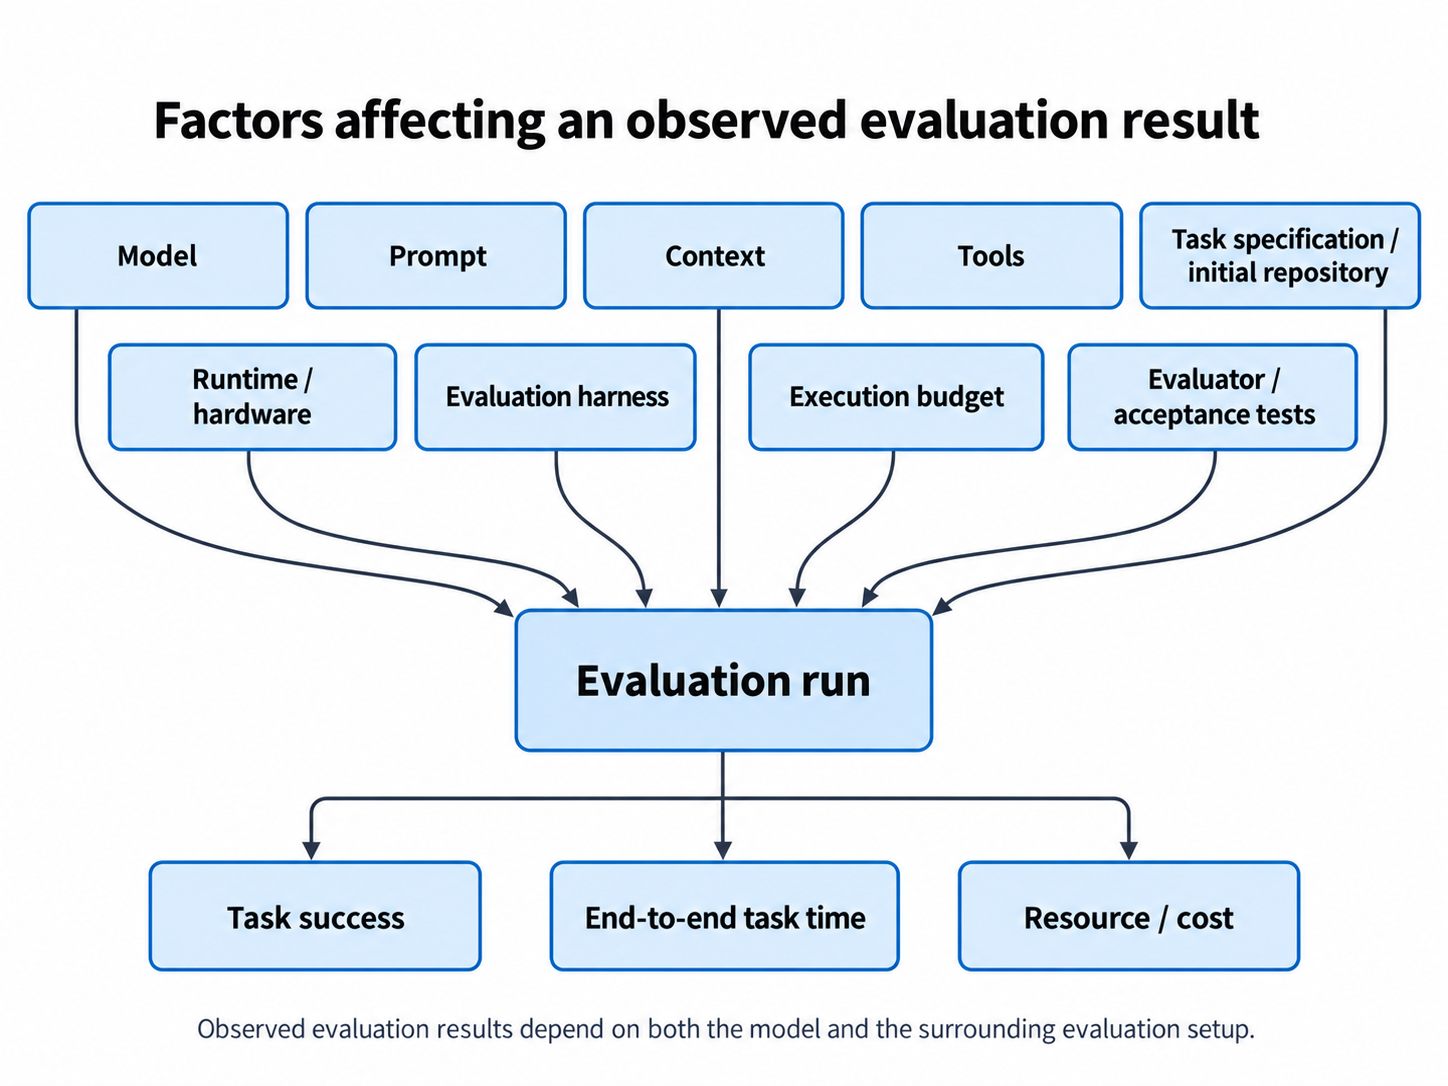
\includegraphics[width=14cm,trim=0 45bp 0 60bp,clip]{images/evaluation-result-factors.png}
\captionsetup{hypcap=false}
\captionof{figure}{Factors influencing an observed evaluation result, including the assistant configuration, task conditions, execution environment and independent verification.}
\label{fig:evaluation-factors}
\end{minipage}

Candidate models should therefore be compared under controlled conditions. Each candidate should receive the same task specification, initial repository state, system prompt, context policy, tools and execution budget. One evaluation run may contain several internal actions, such as editing code, running tests and revising a failed solution. A repeated run instead restarts the task from the same initial state. Providing one candidate with additional runs or a larger execution budget would make the results less comparable.

\section{Reliability and limitations of LLM evaluation}
\label{sec:evaluation-limitations}

Benchmark scores remain imperfect measurements. Saturation reduces their ability to distinguish advanced models, while data contamination can occur when public benchmark tasks later appear in training corpora. Evaluation results may also vary between runs because LLM generation can be stochastic. Small differences should therefore be interpreted cautiously, and the number of evaluated tasks and repeated runs should be reported where relevant.

Tasks used to tune prompts, context strategies or other parts of the assistant should also be separated from those used for final comparison. Otherwise, the system may become indirectly optimised for its own evaluation set.

A further limitation is evaluator validity. Execution-based evaluation is stronger than judging whether generated code merely appears plausible, but passing tests is meaningful only when the specification and tests correctly represent the intended behaviour. A 2026 audit of the 731-task public SWE-Bench Pro split illustrates this problem. After an automated filter identified potentially problematic tasks, OpenAI reported breaking evaluation issues in 200 tasks through a human-supervised agent audit and in 249 tasks through human annotation, corresponding to 27.4\% and 34.1\% of the full public split \parencite{openai2026codingaudit}. Reported problems included underspecified requirements, tests enforcing unstated implementation details, insufficient test coverage and conflicts between task descriptions and evaluators.

Such problems can produce errors in both directions: a valid implementation may fail because an evaluator checks an unstated requirement, while an incomplete implementation may pass because relevant behaviour is not covered. Execution-based evaluation is therefore only as reliable as its task specification and test suite.

The same principle should apply to an internal evaluation of the assistant. Task descriptions and acceptance criteria should be reviewed before comparison, and final verification should use fixed evaluation tests that the assistant cannot modify. Ambiguous outcomes should be checked against predefined acceptance criteria.

\section{Model selection for the assistant}
\label{sec:assistant-model-selection}

Public benchmarks should primarily be used to create a shortlist. Deployment constraints from Chapter~\ref{chap:local-llms} can first exclude configurations that do not satisfy hardware or runtime requirements. Relevant reasoning, coding and software-engineering benchmarks can then provide preliminary evidence about the remaining candidates.

The final comparison should use representative repository-level tasks, such as bug fixing, API changes, database validation, refactoring and coordinated multi-file modifications. Candidate configurations should be evaluated under the same task, environment and execution conditions defined in Section~\ref{sec:engineering-capabilities}.

Task success should be the primary quality metric. A successful task should require the requested behaviour to be implemented, predefined acceptance tests to pass and existing regression tests to remain successful. Results should also be examined by task category, since two candidates with similar overall success rates may fail on different types of work.

Operational metrics provide additional information once candidates satisfy the required quality level. End-to-end task time is more relevant than time to first token for workflows involving repository inspection, multiple model calls and repeated test execution. Completion time should be interpreted together with task success, with failed runs and timeouts reported separately. Resource measurements should cover the complete evaluation run, including model inference and tool execution. For API-hosted models this may include token or request cost, while local configurations can instead be compared using hardware utilisation, execution time or an explicitly defined compute cost. Any cost-per-success metric should also include resources consumed by failed runs.

Model selection should therefore follow predefined requirements rather than simply choosing the highest benchmark score. Candidates that fail the required quality or deployment constraints should be excluded; the remaining configurations can then be compared using task success, completion time and resource consumption.

This chapter defines the criteria and procedure for a preliminary model shortlist rather than selecting a final model in isolation. Final selection requires testing the remaining candidates within the assistant's actual tool, context and interaction architecture, which is developed in the following chapters.
